\documentclass [11pt,twoside]{article}
\usepackage[utf8]{inputenc}
\usepackage[T1]{fontenc}

%Page margins, header and footer positions
\usepackage{geometry}
 \geometry{
 a4paper,
 total={210mm,297mm},
 left=25mm,
 right=25mm,
 top=30mm,
 bottom=25mm,
 headsep=7mm}

\interfootnotelinepenalty=10000

%To display filling dots in the TOC for all entries
\usepackage[titles]{tocloft}
\renewcommand{\cftsecleader}{\cftdotfill{\cftdotsep}}

%Define new header and footer style
\usepackage{fancyhdr}

\pagestyle{fancy}
\fancyhf{}
\lhead{\color{Gray}{\small{SafeStreet Project - Maldini , Paone}}}
\lfoot{\textcolor{Gray}{\small{Copyright © 2019, Maldini, Paone – All rights reserved}}}
\rfoot{\textcolor{Gray}{\thepage}}
\renewcommand{\headrulewidth}{0pt}

%PACKAGES
\usepackage{wasysym}
\usepackage{pifont}

\newcommand{\supported}{\ding{52}\xspace}
\newcommand{\unsupported}{\ding{55}\xspace}
\newcommand{\partsupported}{\textcolor{black!40}{\ding{52}}\xspace}
\newcommand{\lowsupported}{\textcolor{black!20}{\ding{52}}\xspace}
\newcommand{\unknowsupported}{\textbf{?}\xspace}

%Font: Times
\usepackage{times}
%Change monospaced font
\renewcommand{\ttdefault}{lmtt}

%tables
\usepackage{tabu}
\usepackage{tabularx}
\usepackage{ltablex}
\usepackage{longtable}
\usepackage{float} % To allow the use of H modifier in long tables

%landscape mode
\usepackage{pdflscape}
\usepackage{rotating}
\usepackage{caption}

%make landscape mode be sensitive to even and odd pages
%start
\def\myrotate{\ifodd\c@page\else-\fi 90}
\makeatletter
\global\let\orig@begin@landscape=\landscape%
\global\let\orig@end@landscape=\endlandscape%
\gdef\@true{1}
\gdef\@false{0}
\gdef\landscape{%
    \global\let\within@landscape=\@true%
    \orig@begin@landscape%
}%
\gdef\endlandscape{%
    \orig@end@landscape%
    \global\let\within@landscape=\@false%
}%
\@ifpackageloaded{pdflscape}{%
    \gdef\pdf@landscape@rotate{\PLS@Rotate}%
}{
    \gdef\pdf@landscape@rotate#1{}%
}
\let\latex@outputpage\@outputpage
\def\@outputpage{
    \ifx\within@landscape\@true%
        \if@twoside%
            \ifodd\c@page%
                \gdef\LS@rot{\setbox\@outputbox\vbox{%
                    \pdf@landscape@rotate{-90}%
                    \hbox{\rotatebox{90}{\hbox{\rotatebox{180}{\box\@outputbox}}}}}%
                }%
            \else%
                \gdef\LS@rot{\setbox\@outputbox\vbox{%
                    \pdf@landscape@rotate{+90}%
                    \hbox{\rotatebox{90}{\hbox{\rotatebox{0}{\box\@outputbox}}}}}%
                }%
            \fi%
        \else%
            \gdef\LS@rot{\setbox\@outputbox\vbox{%
                \pdf@landscape@rotate{+90}%
                \hbox{\rotatebox{90}{\hbox{\rotatebox{0}{\box\@outputbox}}}}}%
            }%
        \fi%
    \fi%
    \latex@outputpage%
}
\makeatother
%end

%graphics
\usepackage{graphicx}
\usepackage[dvipsnames, table]{xcolor}
%If you upload images from PC, you need to insert code for the path here (different for Windows and Unix OS)

%References
%\usepackage{xpatch}
%\usepackage[backend=biber, style=numeric, citestyle=numeric, sorting=none]{biblatex}
%\addbibresource{main.bib}

%Other
\usepackage{ifthen}
\usepackage{xspace}
\usepackage{enumitem}
\usepackage{amssymb}
\usepackage[pdftex, colorlinks]{hyperref}
\newcommand{\comment}[1]{{\color{Red}$\blacktriangleright$ Comment: #1 $\blacktriangleleft$}}


% Some utilities\ldots
\usepackage{soul}
\usepackage{tikz}

\usetikzlibrary{calc}
\usetikzlibrary{decorations.pathmorphing}


\makeatletter

\newcommand{\defhighlighter}[3][]{%
  \tikzset{every highlighter/.style={color=#2, fill opacity=#3, #1}}%
}

\defhighlighter{yellow}{.5}

\newcommand{\highlight@DoHighlight}{
  \fill [ decoration = {random steps, amplitude=1pt, segment length=15pt}
        , outer sep = -15pt, inner sep = 0pt, decorate
       , every highlighter, this highlighter ]
        ($(begin highlight)+(0,8pt)$) rectangle ($(end highlight)+(0,-3pt)$) ;
}

\newcommand{\highlight@BeginHighlight}{
  \coordinate (begin highlight) at (0,0) ;
}

\newcommand{\highlight@EndHighlight}{
  \coordinate (end highlight) at (0,0) ;
}

\newdimen\highlight@previous
\newdimen\highlight@current

\DeclareRobustCommand*\highlight[1][]{%
  \tikzset{this highlighter/.style={#1}}%
  \SOUL@setup
  %
  \def\SOUL@preamble{%
    \begin{tikzpicture}[overlay, remember picture]
      \highlight@BeginHighlight
      \highlight@EndHighlight
    \end{tikzpicture}%
  }%
  %
  \def\SOUL@postamble{%
    \begin{tikzpicture}[overlay, remember picture]
      \highlight@EndHighlight
      \highlight@DoHighlight
    \end{tikzpicture}%
  }%
  %
  \def\SOUL@everyhyphen{%
    \discretionary{%
      \SOUL@setkern\SOUL@hyphkern
      \SOUL@sethyphenchar
      \tikz[overlay, remember picture] \highlight@EndHighlight ;%
    }{%
    }{%
      \SOUL@setkern\SOUL@charkern
    }%
  }%
  %
  \def\SOUL@everyexhyphen##1{%
    \SOUL@setkern\SOUL@hyphkern
    \hbox{##1}%
    \discretionary{%
      \tikz[overlay, remember picture] \highlight@EndHighlight ;%
    }{%
    }{%
      \SOUL@setkern\SOUL@charkern
    }%
  }%
  %
  \def\SOUL@everysyllable{%
    \begin{tikzpicture}[overlay, remember picture]
      \path let \p0 = (begin highlight), \p1 = (0,0) in \pgfextra
        \global\highlight@previous=\y0
        \global\highlight@current =\y1
      \endpgfextra (0,0) ;
      \ifdim\highlight@current < \highlight@previous
        \highlight@DoHighlight
        \highlight@BeginHighlight
      \fi
    \end{tikzpicture}%
    \the\SOUL@syllable
    \tikz[overlay, remember picture] \highlight@EndHighlight ;%
  }%
  \SOUL@
}

\makeatother

% Common abbrev. are set as commands to ensure proper spacing after the dot
\RequirePackage{xspace}
\newcommand{\ie}{i.e.\@\xspace}
\newcommand{\aka}{a.k.a.\@\xspace}
\newcommand{\Ie}{I.e.\@\xspace}
\newcommand{\cf}{cf.\@\xspace}
\newcommand{\Cf}{Cf.\@\xspace}
\newcommand{\eg}{e.g.\@\xspace}
\newcommand{\Eg}{E.g.\@\xspace}
\newcommand{\etal}{et al.\@\xspace}
\newcommand{\etc}{etc.\@\xspace}
\newcommand{\wrt}{w.r.t.\@\xspace}
\newcommand{\Wrt}{W.r.t.\@\xspace}



\date{}



\usepackage{eso-pic,graphicx}
\usepackage{float}
\usepackage[dvipsnames]{xcolor}
    \usepackage{listings}

\usepackage{hyperref}
\hypersetup{colorlinks,breaklinks,linkcolor=black,urlcolor=blue}
\begin{document}

%TITLE PAGE

\begin{titlepage}




{\begin{table}[t!]
\centering
\begin{tabu} to \textwidth { X[1.3,r,p] X[1.7,l,p] }
\textcolor{Blue}
{\textbf{\small{Computer science and engineering Software engineering 2 - Project 2019/2020}}} & 
\includegraphics[scale=0.5]{Images/PolimiLogo}
\end{tabu}
\end{table}}~\\ [7cm]


\begin{flushleft}




\end{flushleft}
\AddToShipoutPictureBG*{
\includegraphics[width=\paperwidth,height=\paperheight]{Images/SafeStreets.png}}
\end{titlepage}


\begin{table}[h!]
\begin{tabu} to \textwidth { X[0.3,r,p] X[0.7,l,p] }
\hline

\textbf{Deliverable:} & ATD\\
\textbf{Title:} & Acceptance Testing \\
\textbf{Authors:} & Maldini Pietro , Paone Angelo \\
\textbf{Version:} & 1.0 \\ 
\textbf{Date:} & 21-January-2020 \\
\textbf{Download page:} & https://github.com/pm390/MaldiniPaone\\
\textbf{Copyright:} & Copyright © 2019, Maldini Pietro, Paone Angelo – All rights reserved \\
\hline
\end{tabu}
\end{table}




\setcounter{page}{2}


%------------------------------------------------------------------------------------------------------------------------------------------------
\newpage
\addcontentsline{toc}{section}{Table of Contents}
\tableofcontents


%------------------------------------------------------------------------------------------------------------------------------------------------
\clearpage
{\color{Blue}{\section{Introduction}}}
\label{sect:introduction}

%---------------------------------------------------
\subsection{Purpose}
This document represents the Requirement Analysis and Specification Document (RASD). Goals of
this document are to completely describe the system-to-be in terms of functional and non-functional
requirements, analyse the real needs of the users in order to model the system, show the constraints
and the limit of the software and indicate the typical use cases that will occur after the release. This
document is addressed to the developers who have to implement the requirements and could be used as
a contractual basis. 
%---------------------------------------------------
\subsubsection{Goals}
\begin{itemize}
\item	USER:
\begin{itemize}
\item[G1] Notify authorities about traffic violations
\begin{itemize}
\item[G1-1] Send picture of violation
\item[G1-2] Send Position of the violation
\end{itemize}
\item[G2]Authorities must be able to take an available assignment
\item[G3] Allow authorities to report a finished assignment
\item[G4]Allow all actors to visualize update statistics
\item[G5] Allow the system manager to register Municipality to the service
\end{itemize}
\item	SafeStreets:
\begin{itemize}
\item[G6] Allow a Visitor to join the system registering him/herself to ensure reliability of the information provided by him/her
\item[G7] Store information about violations provided by users:
\begin{itemize}
\item[G7-1] Complete it with metadata
\item[G7-2] Mine information
\end{itemize}
\item[G8] Identify potentially unsafe areas:
\begin{itemize}
\item[G8-1] Suggest possible interventions
\end{itemize}
\item[G9] Allow municipality to register Authorities to the service
\end{itemize}
\item	Security Goals:
\begin{itemize}
\item[S1] Offer different levels of visibility to different type of users
\item[S2] Personal data of users are stored respecting current security standards
\end{itemize}
\end{itemize}
%---------------------------------------------------
\subsection{Scope}
\subsubsection{Description of the given problem}
SafeStreets is a crowd-sourced application whose intention is to notify the authorities when traffic
violations occur. Citizens, thanks to the system, will be able to send information about violations to the
authorities who will take actions against them. In this way, the service provided by the authorities can be
improved because they will receive notifications through the app. The sources of notifications are the
Citizens who take photos of violations and send them to the authorities through
the application. The information provided by users are integrated with other suitable information and are
stored by the service. The system also runs an algorithm to read the license plate of the vehicle in the
photos. All collected data can be seen by Citizens and authorities to find which streets are the safest.
Users can have different levels of visibility: authorities must be able to know the license plates of vehicles
in the photos, while normal users can only see data in the form of statistics. Moreover, data are sent to
the municipal district so that important information can be extracted through statistics in order to make
decisions to improve the safety of the area. Finally, the system will have to be easy to use, reliable
and highly scalable to fit perfectly with the mutable context in which it will be used.

%---------------------------------------------------
\subsubsection{Phenomena}
\begin{itemize}
\item
World phenomena:
\begin{enumerate}
\item
Violation
\item
Intervention of authorities
\item
Municipality put into effect interventions to improve safety
\end{enumerate}
\item
Machine phenomena:	
\begin{enumerate}
\item
Shortest path calculation for authority’s intervention (done by mapping system)
\item
the creation of an object of type violation
\item
run algorithm to identify the license plate/s in the photos
\item
schedule most efficient path to look up the notified violations
\item
periodically run algorithm to suggest possible interventions to municipality
\end{enumerate}
\item
Shared phenomena:
\begin{enumerate}
\item
user notify the system about violation (observed by the system controlled by the world)
\item
send notification to authorities (controlled by system observed by world)
\end{enumerate}
\end{itemize}
%---------------------------------------------------
\subsection{Definitions, Acronyms, Abbreviations}
\subsubsection {Definitions}
\begin{itemize}
\item	Violation: parking violations which can be notified by Citizens to authorities
\item	Report: Notification sent by Citizens to the system
\item	Mapping System: external software that provides maps and directions to reach the position of a violation
\item	Licence plate Recognition Algorithm: calculation process that identifies the alphanumeric number on license plate
\item	Spam: a series of messages that are undesired
\item	App: application software 
\item	Blocked: means that the account is banned for a given period
\item	Metadata: data about a violation. Position , date,  time and the username of Citizen. 
\item	Assignment : Work Request for authorities generated upon the receiving of a notification made by Citizens.
\end{itemize}
%---------------------------------------------------
\subsubsection {Acronyms}
\begin{itemize}
\item	RASD: Requirement Analysis and Specification Document.
\item	API: Application Programming Interface
\item	GPS: Global positioning system
\item	HTTP: HyperText Transfer Protocol
\item	HTTPS: HyperText Transfer Protocol over Secure Socket Layers
\item	UML: Unified Modeling Language

\end{itemize}
%---------------------------------------------------
\subsubsection {Abbreviations}
\begin{itemize}
\item	[Gn]: n-th goal.
\item	[Dn]: n-th domain assumption.
\item	[Rn]: n-th requirement.
\item     Municipality: municipal employee.
\end{itemize}
%---------------------------------------------------
\subsection {Revision History}
\begin{itemize}
\item      RASDv1.0 felivered on 10/11/2019: first delivery.
\item	RASDv2.0 delivered on 15/12/2019 : TODO write what we modified
\end{itemize}
%---------------------------------------------------
\subsection {Reference Documents}
\begin{itemize}
\item	Specification Document: “Assignments AA 2019-2020.pdf”.
\item	\href{http://homepage.cs.uiowa.edu/~tinelli/classes/181/Spring10/Notes/09-dynamic-models.pdf }{Alloy Dynamic Model example} 
\item	IEEE Std 830-1993 - IEEE Guide to Software Requirements Specifications.
\item	IEEE Std 830-1998 - IEEE Recommended Practice for Software Requirements Specifications.

\end{itemize}
%---------------------------------------------------
\subsection{Document Structure}
This chapter debates about contents and structure of RASD, indeed this document, based on standards IEEE, is divided in six different sections:
\begin{enumerate}
\item	The Introduction provides a general appearance of the systems defining which are the goals to reach, describing the problem and introducing the world and shared phenomena.
\item The Overall Description provides the description of the relevant components that system needs, the involved actors’ characteristics, and the assumptions to better clarify the needs and the boundaries of the system. 
\item Specific Requirements contains the goals, the functional and non-functional requirements of the system are presented. In addition, a mock-up representation of the application expslain and gives a feeling on how the app will look like and show the main actions it can perform.
\item Scenarios describe the usefulness of SafeStreet and its features in some situations that could happen.
\item UML Modelling contains the diagrams that are referred to the functionality of the system, they explain the workflow of some scenarios, the actions and the structure of the actors and the state that system assumes. These features are represented by Use Case diagram, Sequence diagram, Class diagram and Activity diagram.
\item Alloy Modelling allows to explain the world models through Alloy model of system. The mockups generated by the Alloy modelling grants that, given requirements and domain assumption, the goals are satisfied.

\end{enumerate}


%------------------------------------------------------------------------------------------------------------------------------------------------
\clearpage
{\color{Blue}{\section{Setup}}}
\label{sect:Setup}
%.-------------------------------------------------------------------------------------------------------------------------------------------------------------
\subsection{Back-end setup}
%.-------------------------------------------------------------------------------------------------------------------------------------------------------------
In this phase of setup, it is required a software called docker that could be preinstalled. The installation process of this prerequisites should be explained because, during this configuration part we have found some complications: 
At first time, we’ve tried to install docker provided from the official web site but, the installation is interrupted, because Docker Desktop requires Windows 10 Pro or Enterprise version 15063 to run, therefore the versions of the operating system of our devices can’t guest the software. At second time, after consulting of forum web site we have found on https://github.com/docker/toolbox/releases the installer that could by pass the prerequisites of the operating system version. We have downloaded DockerToolbox-19.03.1.exe and we’ve executed it and done the full installation setup. After that, we have run the Docker Quickstart Terminal which during his initial setup it have downloaded some files, when finished his initial phase we have copied the docker-compose.yml from package given by the other team (… -> DeliveryFolder -> implementation -> back) and pasted to the folder of Docker Toolbox (C: Program Files -> Docker Toolbox). Subsequently  we have run the command “docker-compose up”, on docker terminal, (indicated in the section 6 from ITD document) and when docker have finished his set up, we have tested on the browser the link given by the other team http://localhost:8080/auth/ping having a successful result.  Immediately we have tried to connect the mobile app but without success and then we have created and executed a file.bat which use “NETSH PORTPROXY” command to create a bridge from virtual machine to subnet and then we have tried again to establish the connection with mobile app having a successful result.

%.-------------------------------------------------------------------------------------------------------------------------------------------------------------
\subsection{Front-end setup}
In this phase of setup, we have followed the instructions (indicated in the section 6 from ITD document) with a successful result about the installation of mobile app.
%.-------------------------------------------------------------------------------------------------------------------------------------------------------------
\subsubsection{Setup conclusion}
The ITD1.pdf has a lack of explanation abouth the installation process of the back-end, some instructions should be given in case of a non compatibility of the system with the prerequisite software which should be installed.











%------------------------------------------------------------------------------------------------------------------------------------------------
\clearpage
{\color{Blue}{\section{Acceptance tests}}}
\label{sect:Acceptance tests}
%.-------------------------------------------------------------------------------------------------------------------------------------------------------------
\subsection{Acceptance tests}
%.-------------------------------------------------------------------------------------------------------------------------------------------------------------
This acceptance tests are based on the use cases located inside the RASD document provided by the other team are respected.
\begin{figure}[H]
\centering
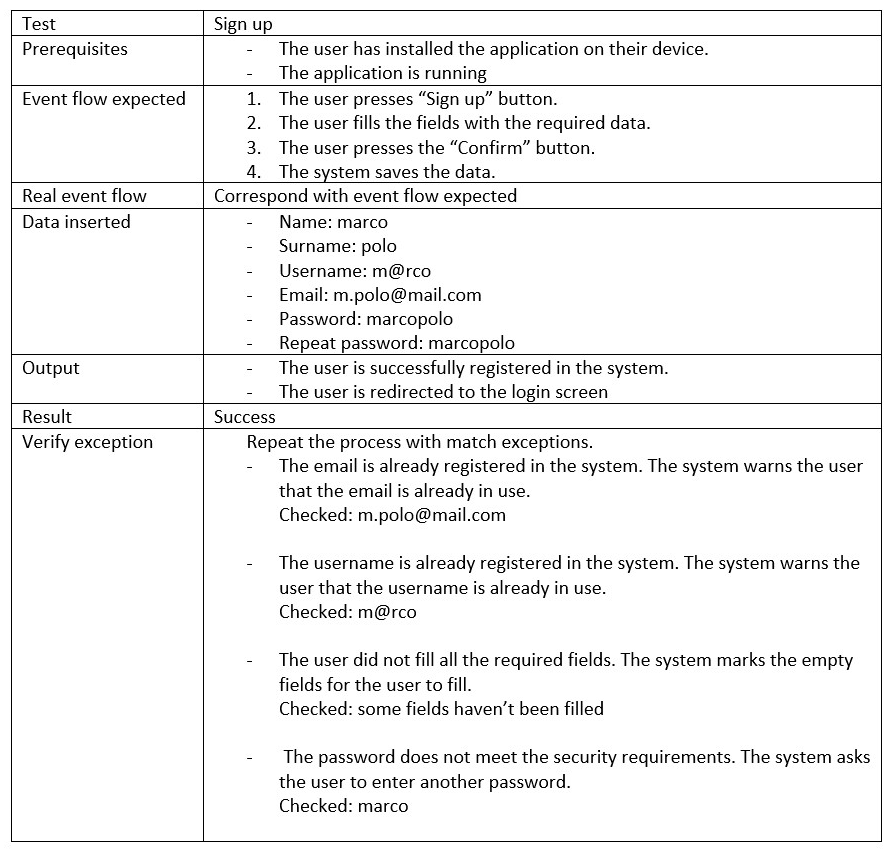
\includegraphics[width=\textwidth]{Images/signup.png}
\end{figure}
\newpage
\begin{figure}[H]
\centering
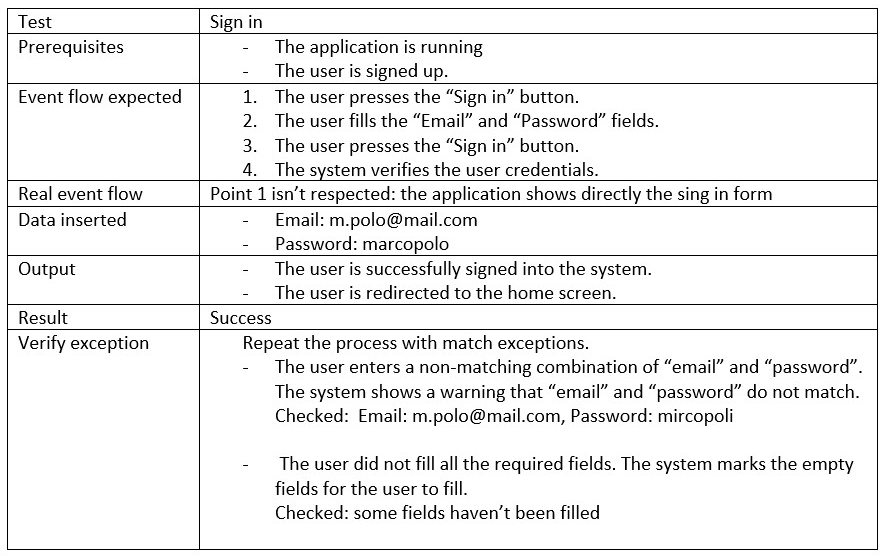
\includegraphics[width=\textwidth]{Images/signin.png}
\end{figure}
\begin{figure}[H]
\centering
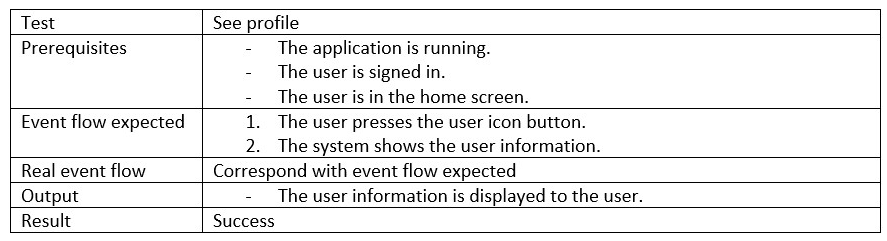
\includegraphics[width=\textwidth]{Images/seeprofile.png}
\end{figure}
\newpage
\begin{figure}[H]
\centering
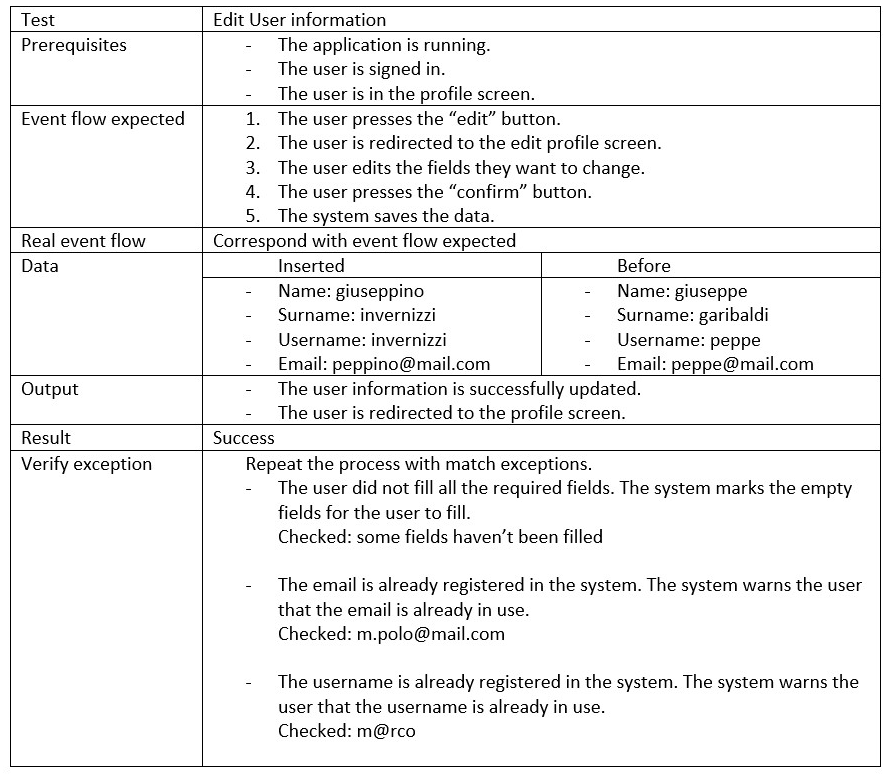
\includegraphics[width=\textwidth]{Images/edituserinformation.png}
\end{figure}
\newpage
\begin{figure}[H]
\centering
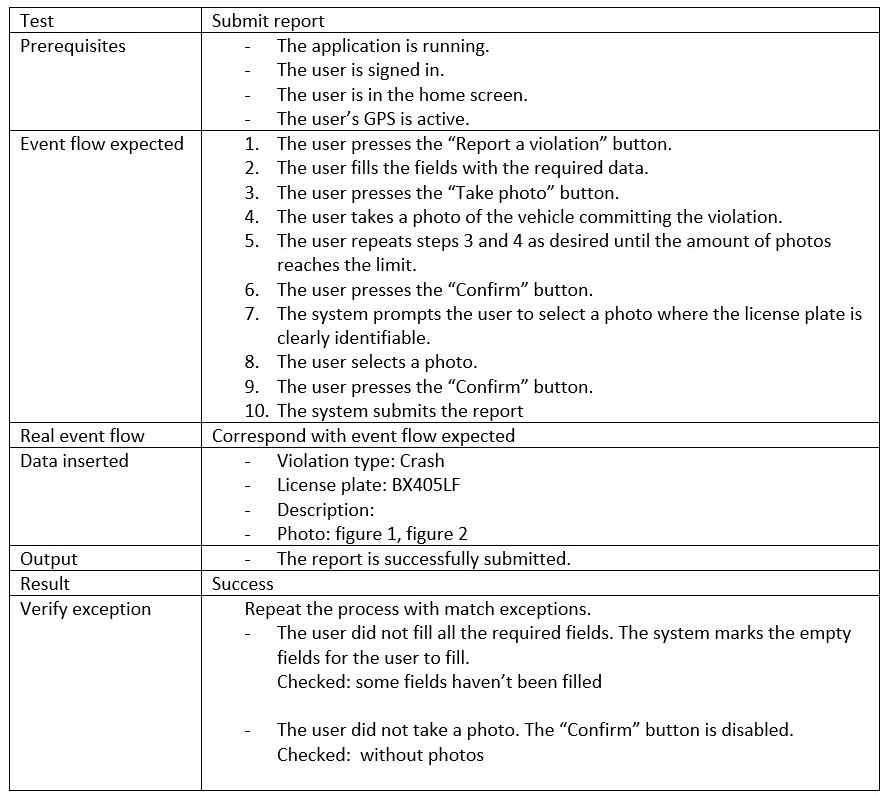
\includegraphics[width=\textwidth]{Images/submitreport.png}
\end{figure}
\begin{figure}[H]
\centering
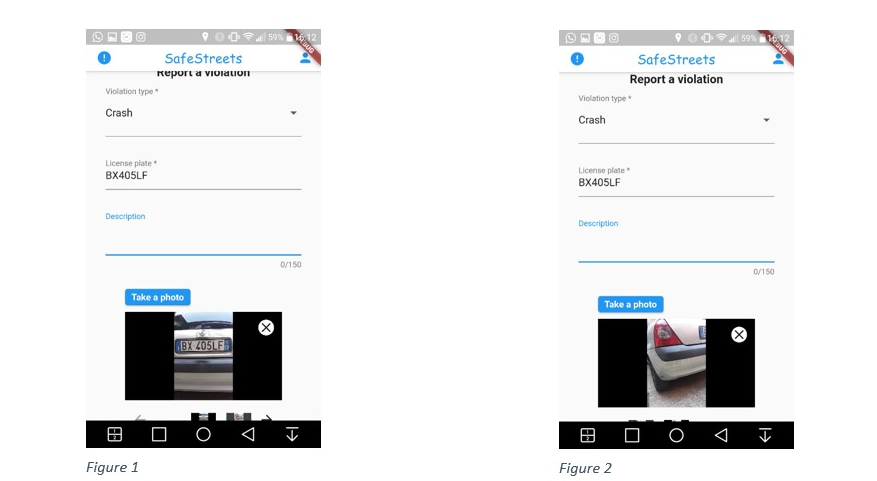
\includegraphics[width=\textwidth]{Images/figure1.png}
\end{figure}
\newpage
\begin{figure}[H]
\centering
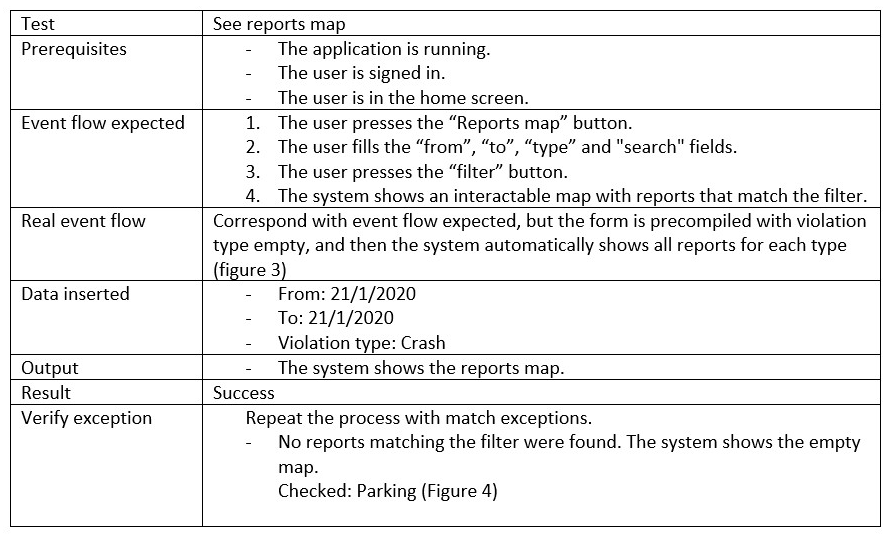
\includegraphics[width=\textwidth]{Images/seereportsmap.png}
\end{figure}
\begin{figure}[H]
\centering
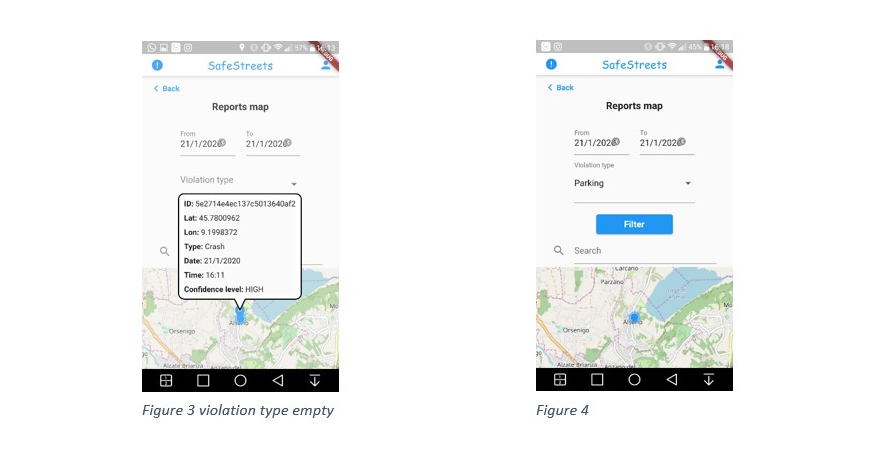
\includegraphics[width=\textwidth]{Images/figure2.png}
\end{figure}











%------------------------------------------------------------------------------------------------------------------------------------------------
\clearpage
{\color{Blue}{\section{Other aspects to consider}}}
\label{sect:Other aspects to consider}
%.-------------------------------------------------------------------------------------------------------------------------------------------------------------
This section presents an analysis of the usability of the project. This section should be considered as suggestions for a further release, some ideas and hints to increase the user experience.
\subsection{Mobile Application Testing}
The application is well structured and provides a good environment to test out the functionalities of the system.
Some functions may be changed to simplify testing :
\begin{itemize}
\item Save last connected ip address: when closing the application the ip gets deleted and the default ip is automatically inserted and used to connect to the server. This slows down testing of behaviour of the application for example testing the behaviour of closing it and reopening it. If the mobile phone is set so that application in background are stopped the ip must be reinserted to make the application communicate with the right ip.
\item Make the Camera choosable: when testing the application having a fixed camera can cause unexpected and undesirable problems. On some phones the primary camera is the internal camera. This caused our testing phase of report making really difficult since we had to make clear photos of the cars and license plates. That was quite a difficult task since internal camera's makes photos with less quality and are usually focused on taking a photo of a person not of a car which can be really big and this reduces too the accuracy of the photo making the testing almost impossible since most photos gets rejected.
\end{itemize}
An additional point is that the interface is really good looking at first glance but seems to be tested only on a certain specific type of screens. Because some screens shows some really bad looking overflow messages for email addresses of accounts which were already available in the database provided.
//TODO photo here

\subsection{Mobile Application for Users}
Here we present some ideas and hints to improve user experience for final users and some improvements to the functionalities to make them more clear and usable:
\begin{itemize}
\item Making the License plate input field Auto Capitalizing : The application for making a report requires the user to manually input the license plate of a violation. The input is not accepted if letters are in lower case, but since the input is a normal text input a normal phone keyboard capitalizes the first letter and puts the other letters in lowercare. This can slow down the creation of a report , the input field may set programmatically the capitalization of the letters inside the license plate. Another way to handle this problem could be just modifying to uppercase all the letters in the license plate server side or client side indifferently.
\item Taking a photo with a camera of choice : The possibility of choosing the camera to take a photo on a phone is required to make the process as easy as possibile for all possible users on the most different devices as possible. 
\item Check overflow behaviour of components : A fixed behaviour should be decided for overflowing elements and texts. Making buttons proportional to the screen size and making text size also proportional to the size may be a possible choice, making scrollbars to see overflowing elements is also a possible behaviour to handle overflows.
\item Top Left Alert button : the button which gives the possibility to review a photo and increase reliability of a report should be visible only if there is a real report to be reviewed. Otherwise for a user which doesn't know how it works may see it and click it several time getting no feedback from the application. Another possibile way to avoid this unexplained button may be setting a default screen pop-up telling the user that there are no reports to be reviewed. Explaining this way the meaning of the component in the user interface.
\item Expect the unexpected : On the report map screen there is a map where the violations are shown with their id , their date and type. In this screen it is possible using a menu to choose to filter violations. The filtering used properly works really well. it is possible to delete the starting or ending date of the filtering . If a user deletes one date of the two and presses filter the screen shows a loading icon on bottom left and after several minutes of loading no responses seems to arrive from the server. Filter should be disabled if both dates are not available or a default date should be decided for both fields. For example one week before as default starting date and the current date as default final date. Another unexpected behaviour is that after changing filter options and setting a certain violation type the map reload the violations but if there is another change in the violation type and filter is clicked there is no loading and no changes occur on the map, the changes happens only when the map is moved.
The filter button should be enabled again after a filter option is changed, this functionality may be useful for municipalities, one municipality may want  to know how different violations are located on their territory. Not having the possibility to filter without moving the map can make the experience tedious and less intuitive.
\item Don't make the user learn , give them what they already know : On the report map it is not possible to directly move in direction north-south because vertical scrolling moves a menu on the top of the map. This behaviour is really unexpected by the user and user must learn that to move north-south they must first move a little east-west and keep moving on the screen vertically to actually move in the desired direction. Final users can be really difficult to please and making them learn new behaviours which are not compatible with behaviours they already are familiars with can really make the difference from a used and a not used application. To fix this issue a button may be placed on top of the screen to make the menu appear or as an alternative an area which is easily recognizable may be put on top and dragging this area makes the menu appear and disappear. This way the map itself remains untouched while the experience of the user increases and a more natural interaction with the map is possible.
\end{itemize}
\subsection{Interfaces}
The design of the interfaces in the application is quite clear and there are no distractions from the actual activity of the user which makes the experience of the user linear and creates less space for unexpected behaviours. 
\newline
There is unity between the various components in the screens so every interface has its compoents arranged in a clear way and makes the interactions clear to the user.
\newline
Functionalities are showed on the main screen with a scaling hierarchy ,showing in big the main functionalities which are making reports and accessing the map with the reports and givin less importance to functionalities like reviewing a report and modifying account.
\newline
All the interfaces are have its components placed in such a way to preserve a balance in the screens which improves the user experience.



%------------------------------------------------------------------------------------------------------------------------------------------------


\end{document}
